% !TEX root = ../PhD Thesis.tex
\chapter{cTRAP: identification of candidate causal perturbations from differential gene expression data}
\label{chap:ctrap}

During a 2017 lab retreat in Madeira, we focused our attention to what were the objectives of the lab and what we could provide to the community. One of the ideas seemed easy to do: comparing a custom differential gene expression against a large database of differential expression profiles. The idea was already been discussed in the original paper of CMap and implemented in their online tool at \rurl{clue.io}, but there were issues with their implementation.

The Connectivity Map or CMap \cite{subramanian:2017ul} is a repository of transcriptomic signatures for thousands of genetic (gene overexpression or knockout) and pharmacological perturbations tested in human cancer cell lines. We developed cTRAP (\rurl{bioconductor.org/packages/cTRAP}), an R/Bioconductor package to compare user-provided differential gene expression profiles with those from CMap, allowing to infer putative candidate molecular causes for the observed differences, as well as compounds that may promote or revert them. The comparisons are made based on correlation and gene set enrichment \cite{subramanian:2005wu} approaches.

The associated manuscript (of which I am a co-first and co-corresponding author) is in preparation for submission to an international peer-reviewed scientific journal.

\section{Background}

\section{cTRAP analyses}

From a vector of user-provided differential expression results (e.g. t-statistic values) with respective gene symbols, cTRAP can return a ranked list of similar CMap perturbations or predict targeting drugs. Moreover, cTRAP can also analyse the enrichment of drug sets in a ranked vector of compounds to identify common compound characteristics.

\begin{figure}[!h]
  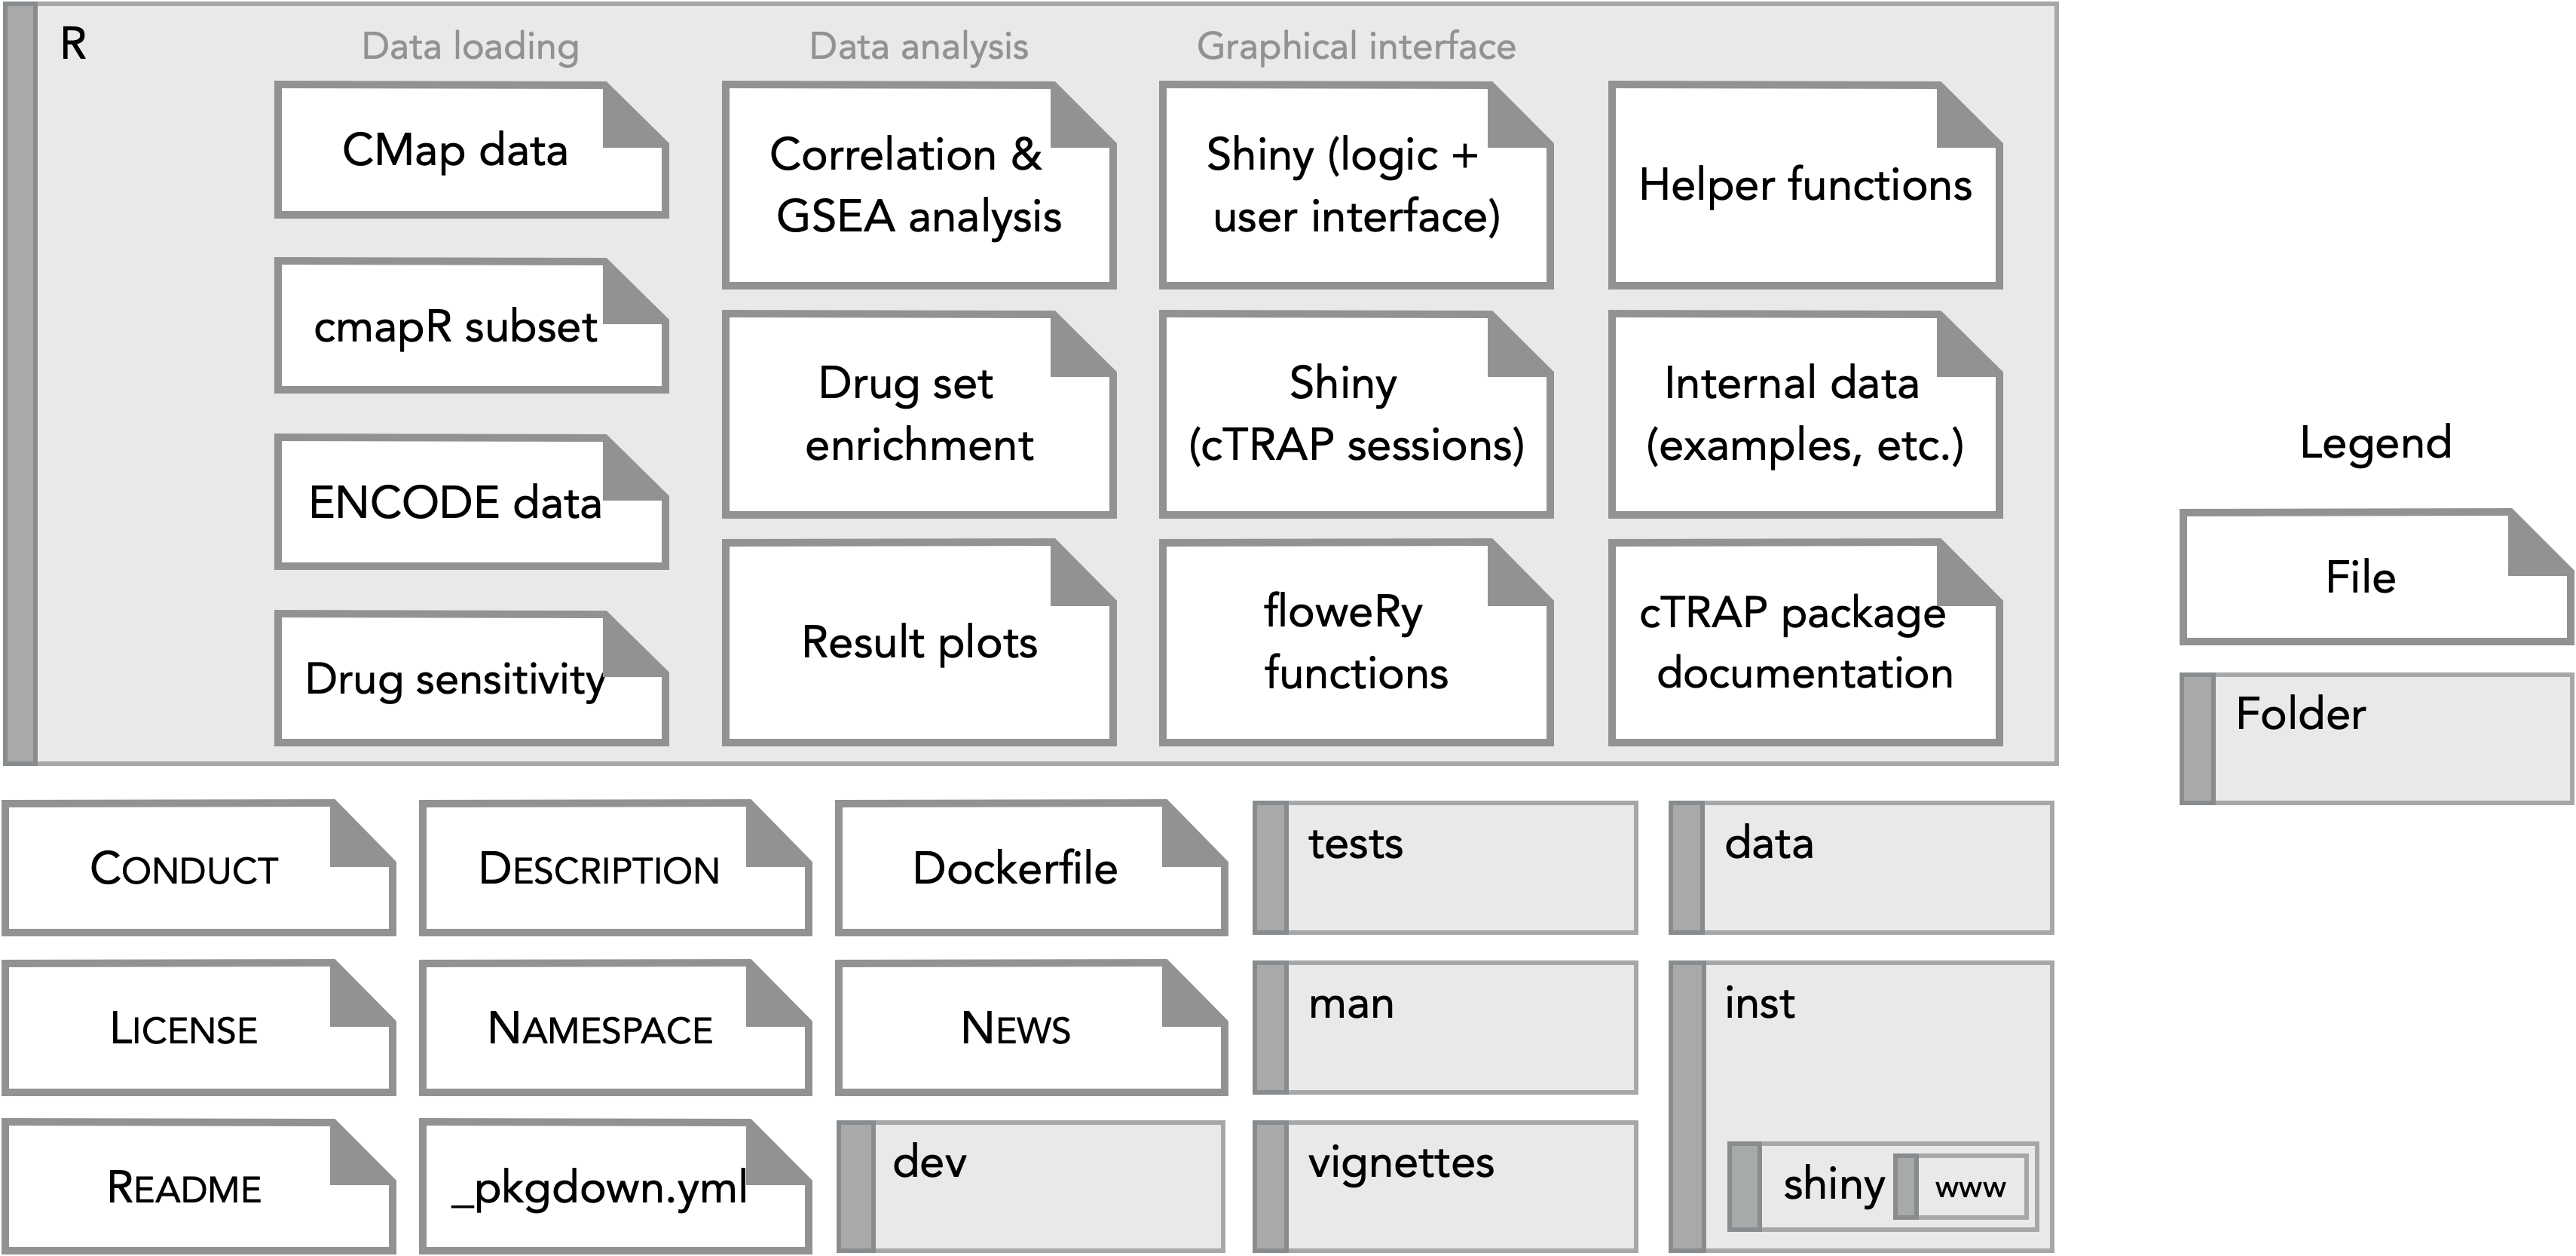
\includegraphics[width=1\textwidth]{images/ctrap/file-structure}
  \centering
  \caption[cTRAP file structure]{\textbf{Visual representation of cTRAP's file structure.} As usual in an R package, the R folder contains the scripts with package functions and data. \texttt{dev} is a non-standard folder for an R package and is only used to store supporting scripts related with cTRAP (e.g. test analyses and benchmarks); contents of the \texttt{dev} folder are not included when building the R package.}
  \label{fig:ctrap-file-structure}
\end{figure}

\subsection{Ranking of similar CMap perturbations}

CMap is a repository of transcriptomic signatures of thousands of genetic and pharmacological perturbations in human cancer cell lines. These perturbations can be categorised into gene knockdown, gene over-expression and compounds. Available perturbation types and respective conditions can be enquired in cTRAP with the function \texttt{getCMapConditions()}, which will download and load CMap perturbation information into R. Afterwards, the function \texttt{filterCMapMetadata()} can be used to download and filter the metadata related to the data to use in downstream analyses based on perturbations types, cell lines, dosages and time points. This information is passed to \texttt{prepareCMapPerturbations()} to download CMap differential expression profiles z-scores (GCTX file) and gene and compound information and load the filtered data only. Note that the GCTX file size is ~21GB and we recommend to download it directly from GEO GSE92742’s Level 5 data link (\sloppy{\small{\url{ftp://ftp.ncbi.nlm.nih.gov/geo/series/GSE92nnn/GSE92742/suppl/GSE92742_Broad_LINCS_Level5_COMPZ.MODZ_n473647x12328.gctx.gz}}}).

\begin{figure}[!h]
  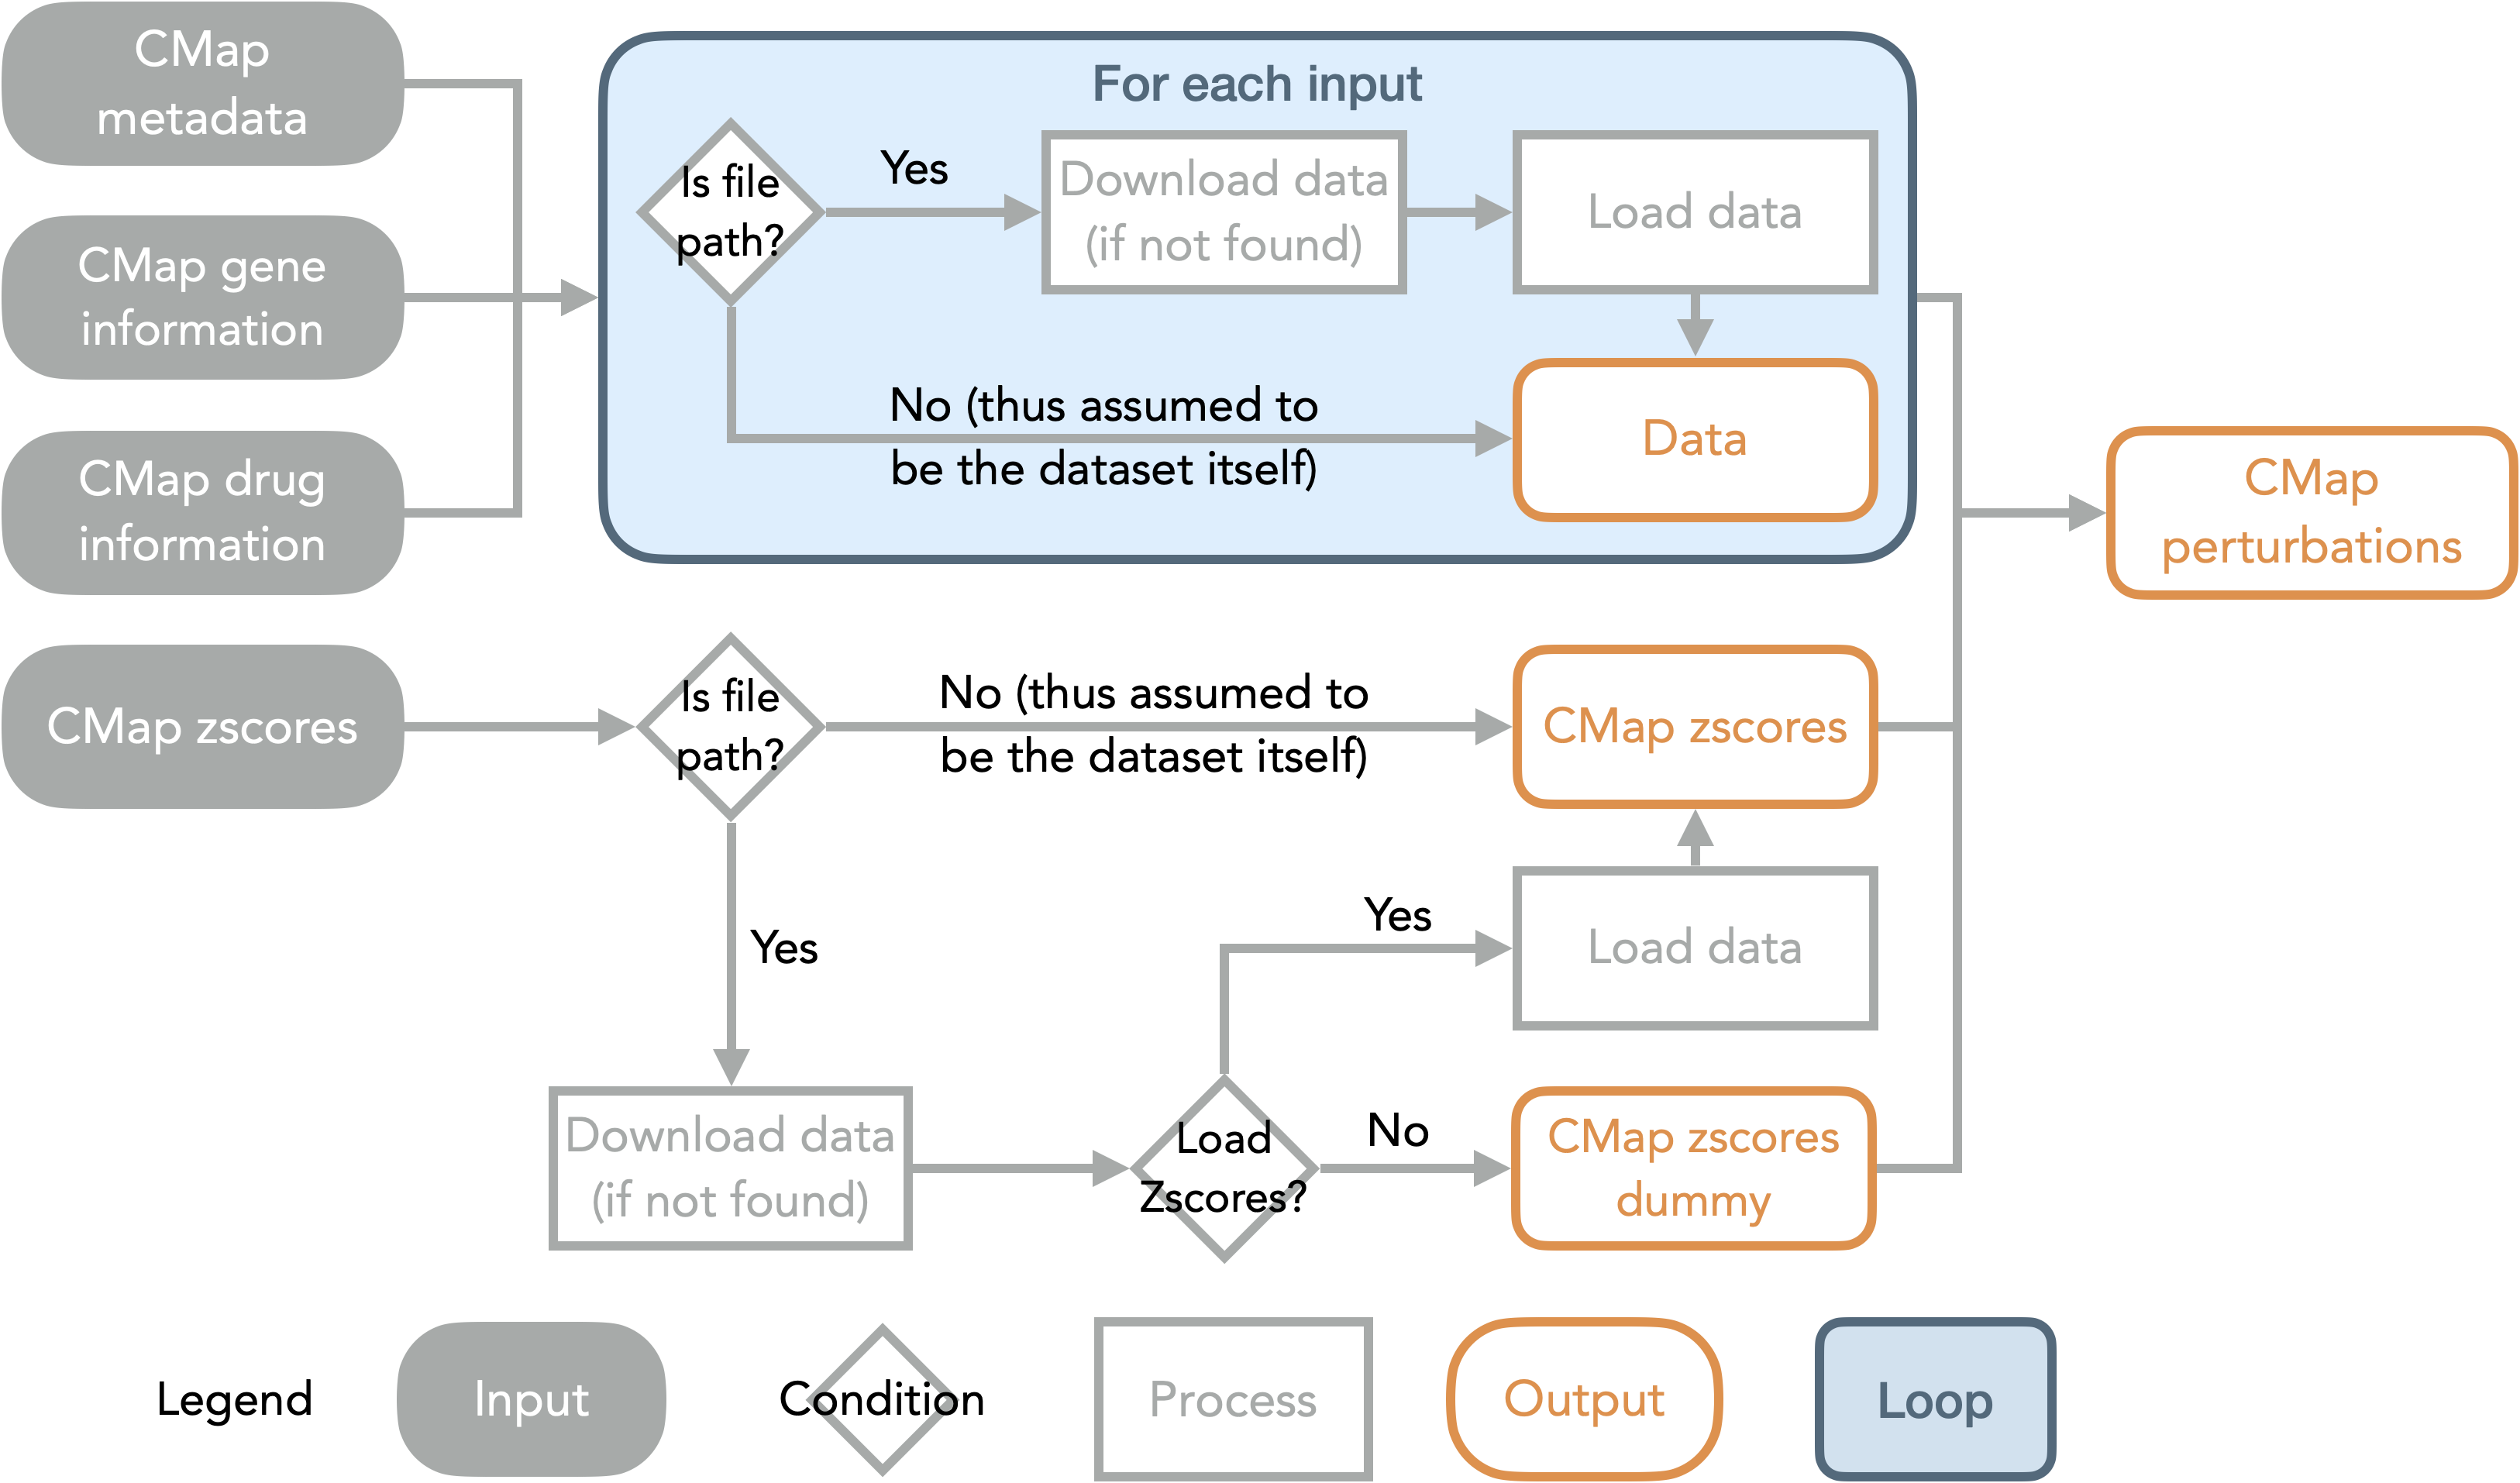
\includegraphics[width=1\textwidth]{images/ctrap/cmap-perturbations}
  \centering
  \caption[Loading data from CMap perturbations]{\textbf{Loading data from CMap perturbations.}}
  \label{fig:ctrap-cmap-perturbations}
\end{figure}

After comparing differential expression z-scores from select CMap perturbations against user-provided differential expression results, \texttt{rankSimilarPerturbations()} returns a table with ranked CMap perturbations and their respective correlation coefficients and GSEA scores. Lower ranks indicate perturbations whose differential expression profiles are more similar to the user-provided data, i.e. CMap perturbations that potentially mimic the user-provided transcriptomic changes, whereas higher ranks define perturbations that may revert those changes.

To rank CMap perturbations, cTRAP performs Spearman's and Pearson's correlations between the user-provided statistics for differential expression and values from CMap perturbations, and calculates a GSEA-based score (all three methods are run by default). For each method, the similarity scores are averaged across multiple cell lines (when available) and the averages are then used to rank CMap perturbations. By default, results for individual cell lines are provided for informative purposes (e.g. to check the heterogeneity of response across cell lines) but not used when ranking. The different ranking scores are combined into one final rank product, finally used to rank the CMap perturbations.

The GSEA-based score is calculated via the following steps:

\begin{enumerate}
	\item Sort genes from the user-provided differential expression statistics;
	\item Define the top 150 (by default) and bottom 150 (by default) genes as two sets
	\item For each CMap perturbation, sort genes by their differential expression z-scores and calculate the Weighted Connectivity Score (WTCS) (1) based on the GSEA enrichment scores for the two sets.
\end{enumerate}

As an example, for a CMap perturbation with a similar differential expression profile to user’s input, we expect to find higher enrichment of the top gene set in the most up-regulated genes and higher enrichment of the bottom gene set in the most down-regulated genes.

To minimise RAM usage, \texttt{prepareCMapPerturbations()} downloads the CMap’s perturbation differential expression z-scores GCTX file (if not previously downloaded) and returns its path without loading the file contents. \texttt{rankSimilarPerturbations()} then loads a chunk of ~1GB or lower from the GCTX file, compares the differential expression z-scores from that chunk against user-provided data and proceeds to loading and comparing the z-scores from the next chunk.

\begin{figure}[!h]
  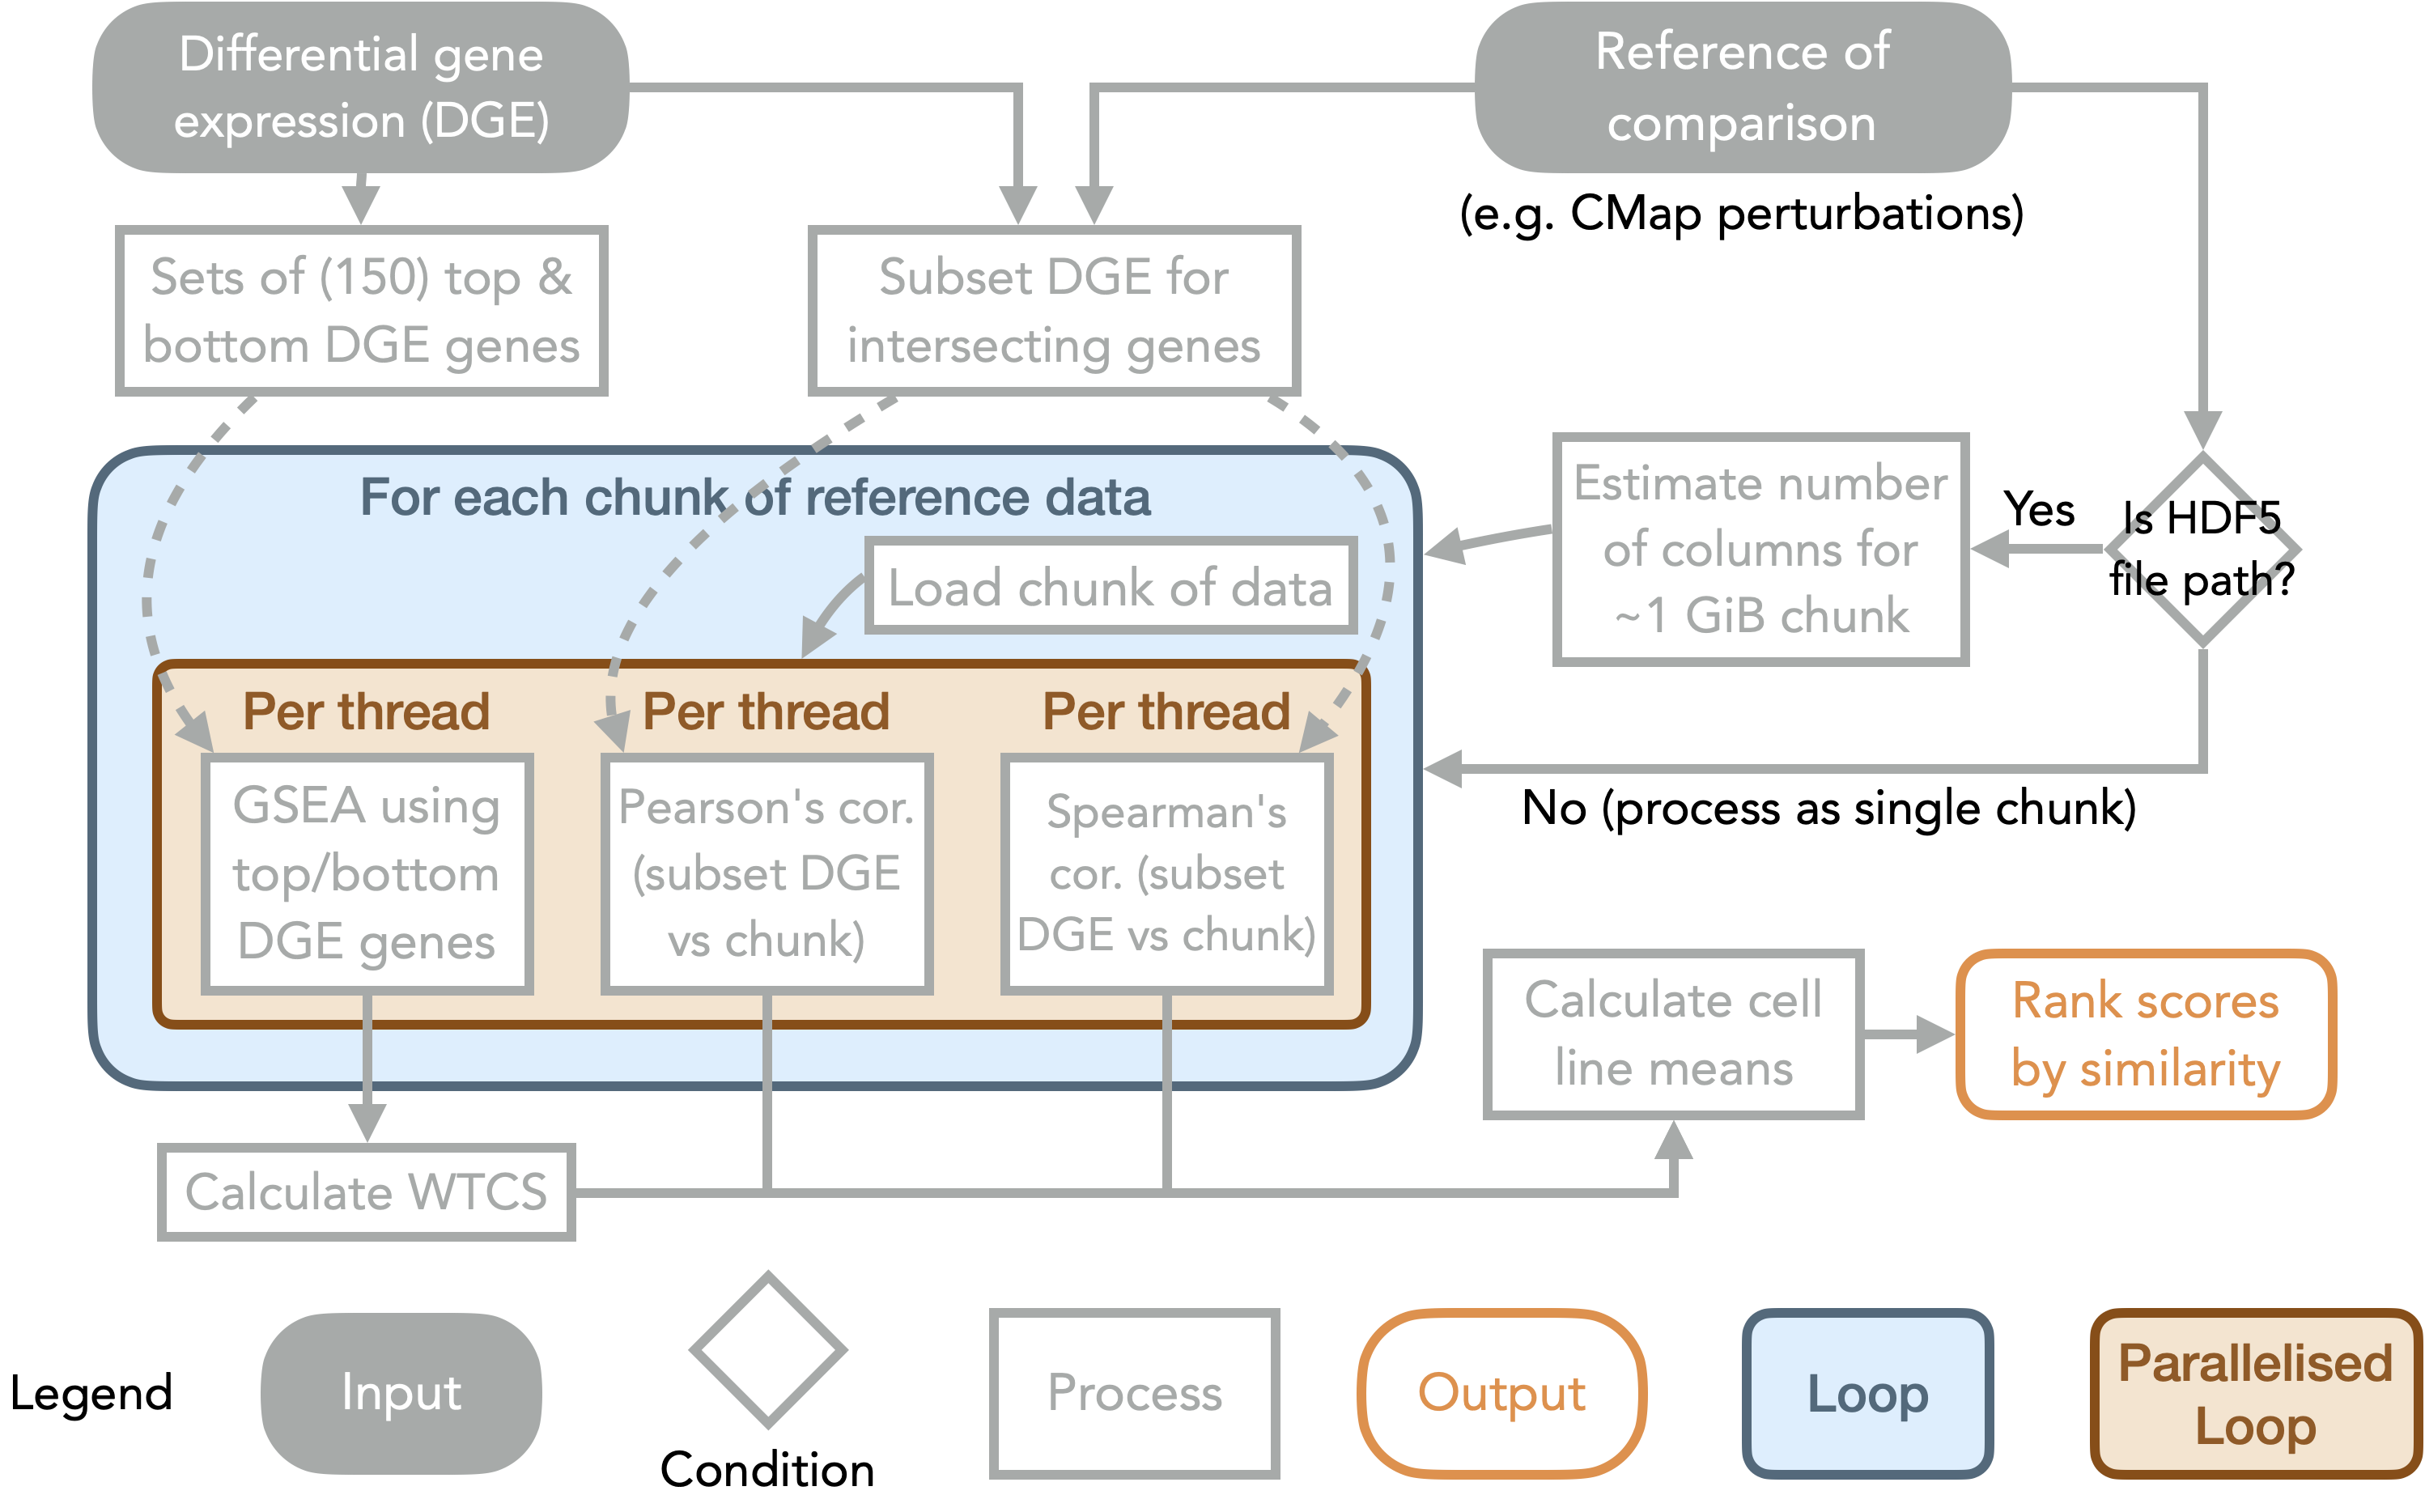
\includegraphics[width=1\textwidth]{images/ctrap/analysis}
  \centering
  \caption[cTRAP analysis workflow]{\textbf{cTRAP analysis workflow}}
  \label{fig:ctrap-analysis}
\end{figure}

The ranked list from \texttt{rankSimilarPerturbations()} can be plotted using \texttt{plot()}, showing a list of all results ordered by a given score or either a scatterplot or GSEA plot for a predicted targeting drug.

\subsection{Prediction of targeting drugs}

Gene expression and drug activity data across multiple cell lines are available from NCI-60 \cite{shoemaker:2006wi}, Cancer Therapeutics Response Portal (CTRP) 2.1 \cite{seashore-ludlow:2015ws} and Genomics of Drug Sensitivity in Cancer (GDSC) 7 \cite{yang:2012vk}. For each source, the internal function \texttt{prepareExpressionDrugSensitivityAssociation()} performs the following steps:

\begin{enumerate}
	\item Download all the necessary data depending on given source;
	\item Perform Spearman’s correlation (by default) between the expression of each gene against the sensitivity of intersecting cell lines to each drug;
	\item Generate a matrix with the correlation coefficients per gene and drug; and
	\item Prepare metadata for downstream analyses, including gene, compound and cell line information from each source.
\end{enumerate}

A higher correlation coefficient for a given gene and drug suggests a gene whose higher expression is associated with higher drug sensitivity across multiple cell lines. As this process can take multiple hours to finish for all sources, the resulting objects were stored online for each aforementioned source and can be listed with \texttt{listExpressionDrugSensitivityAssociation()} and downloaded and loaded into R using \texttt{loadExpressionDrugSensitivityAssociation()}.

To identify compounds that could target the phenotype associated with user-provided differential expression profiles, we use \texttt{predictTargetingDrugs()} with user-provided differential expression results and a correlation matrix of gene expression and drug sensitivity as input. The correlation coefficients between gene expression and drug sensitivity for each drug are compared against user-provided differential expression results by Spearman’s and Pearson’s correlation and GSEA-based scores (as performed when ranking CMap perturbations, results from comparison methods are ranked and then those rankings are finally used to calculate the rank product’s rank). \texttt{predictTargetingDrugs()} returns a table with ranked predicted targeting drugs and their respective correlation coefficients and GSEA scores. A lower rank comprise drugs that may target phenotypes similar to the user-provided differential expression profile.

The resulting object can be plotted with \texttt{plot()}, showing a list of all results ordered by a given score or either a scatterplot or GSEA plot for a predicted targeting drug.

To compare the results from predicted targeting drugs and CMap perturbations that may mimic or revert the observed phenotype, we can use the function \texttt{plotTargetingDrugsVSsimilarPerturbations()}. For the available compound identifiers in the metadata pertaining from the different datasets (e.g. compound name, Broad ID, PubChem CID and SMILES), the function will automatically select the identifiers with higher number of matching values between the two datasets, unless the identifiers are defined. A scatterplot is then plotted using, by default, the rank product’s rank of targeting drugs in one axis and the rank product’s rank of similar perturbations in the other.

\subsection{Drug descriptor set enrichment analysis}

We computed drug descriptors (e.g. molecular weight and number of aromatic rings) for compounds from CMap and NCI-60. The dimensionality of these descriptors can either be 3D (i.e. descriptors calculated based on three-dimensional compound characteristics) or 2D. These datasets are downloaded and loaded into R using \texttt{loadDrugDescriptors()}.

Next, we created sets of descriptors via \texttt{prepareDrugSets()}. By default, the function creates a maximum of 15 sets per drug descriptor. For each alphanumeric descriptor, one set is created per unique value of that descriptor. Alphanumeric descriptors containing more than 15 unique values (by default) will be discarded. For numerical descriptors, \texttt{prepareDrugSets()} internally uses the \texttt{binr::bins()} function to create evenly-distributed bins of drug descriptors, where each set contains a minimum number of points equal to the number of non-missing values divided by the number of maximum sets (15 by default) divided by a constant (5 by default).

By using \texttt{analyseDrugSetEnrichment()}, we analysed the enrichment of the created drug descriptor sets in a named numeric vector or an object returned from \texttt{rankSimilarPerturbations()} – only if run against CMap compound perturbations – or \texttt{predictTargetingDrugs()}. The enrichment analysis is internally performed based on GSEA using \texttt{fgsea::fgsea()}.

The resulting object can be plotted with \texttt{plot()}, showing a list of all results ordered by a given score or either a scatterplot or GSEA plot for a predicted targeting drug.


\section{Benchmarking + code/memory optimisation}

We measured elapsed time using R’s \texttt{Sys.time()} immediately before and after ranking similar CMap perturbations, predicting targeting drugs (using NCI60 expression and drug sensitivity association, the most time-consuming option) and performing drug set enrichment analysis using cTRAP 1.8.1 (296f9b21). As input, we used the t-statistics for the differential expression between EIF4G1 knockdown versus control based on ENCODE gene expression data from cell line HepG2 (the diffExprStat object in the cTRAP package; running \verb|?cTRAP::diffExprStat| shows the R commands to obtain this object).

We measured the heap memory usage of cTRAP 1.8.1 (296f9b21) along time by running R in debug mode with the heaptrack 1.0.0 profiler. heaptrack tracks and logs all calls to the core memory allocation functions via \verb|LD_PRELOAD| and respective backtraces. For R to work properly with heaptrack, the file \path{/usr/bin/R} was edited: all lines of the last \emph{if} statement were commented out with the exception of

\begin{lstlisting}[language=bash,numbers=none]
exec ${debugger} ${debugger_args} "${R_binary}" ${args} "${@}"
\end{lstlisting}

Afterwards, we benchmarked R scripts with:

\begin{lstlisting}[language=bash,numbers=none]
R -d heaptrack -f ${Rscript} --args ${Rscript_args}
\end{lstlisting}

All benchmarks were run in a workstation running Ubuntu 18.04.5 LTS with 768 GB of RAM memory and 72 cores (Intel Xeon Gold 6254 CPU @ 3.10GHz).

\section{Graphical interface}

The most recent feature of cTRAP is its visual interface that allows users to interactively perform most features of cTRAP via the web browser. The graphical interface was modularly built and as an experiment that combines using explicit R commands with an helpful graphical interface. Simply put, there are 5 interface functions:

\begin{itemize}
	\item \texttt{launchDiffExprLoader()} to load differential expression data. Returns a differential expression object that can be used in cTRAP analyses.
	\item \texttt{launchCMapDataLoader()} to explore and load CMap data by type of perturbation, cell types, time points and dosages. Returns filtered CMap data based on the user's selection.
	\item \texttt{launchMetadataViewer()} to check metadata of given cTRAP objects.
	\item \texttt{launchResultPlotter()} to view and plot cTRAP results given as input.
	\item \texttt{launchDrugSetEnrichmentAnalyser()} to analyse drug set enrichment and visualize respective results.
\end{itemize}

Like usual R functions, these graphical interfaces functions accept input and may return output and can thus be intertwined with R code, allowing to easily reproduce cTRAP analyses. For instance:

\begin{lstlisting}[language=R,morekeywords={include, launchDiffExprLoader},keywordstyle=\bfseries]
# Launch differential expression loading interface to select knockdown
# data from ENCODE (pre-filtered for HepG2 cell line and EIF4G1 gene)
diffExpr <- launchDiffExprLoader(cellLine="HepG2", gene="EIF4G1")

# This command does the following:
# 1. Download ENCODE's HepG2 data for EIF4G1 knockdown and controls
# 2. Perform DGE between EIF4G1 knockdown vs. control
# 3. Return resulting t-statistics by gene

# Load CMap knockdown data in HepG2
cmapKD <- launchCMapDataLoader(
    cellLine="HepG2",
    perturbationType="Consensus signature from shRNAs targeting the same gene")
# Load CMap compound data in HepG2
cmapCompounds <- launchCMapDataLoader(cellLine="HepG2",
                                      perturbationType="Compound")
# Load all CMap data in HepG2
cmapPerts <- launchCMapDataLoader(cellLine="HepG2")

# View metadata of all resulting CMap data objects
launchMetadataViewer(cmapKD, cmapCompounds, cmapPerts)

# Rank similar perturbations -----------------------------------------
compareKD        <- rankSimilarPerturbations(diffExpr, cmapKD)
compareCompounds <- rankSimilarPerturbations(diffExpr, cmapCompounds)
comparePerts     <- rankSimilarPerturbations(diffExpr, cmapPerts)


launchResultPlotter(compareCompounds, compareKD, comparePerts)

# Predict targeting drugs --------------------------------------------
listExpressionDrugSensitivityAssociation()
assocMatrix <- listExpressionDrugSensitivityAssociation()[[1]]
assoc       <- loadExpressionDrugSensitivityAssociation(assocMatrix)
predicted   <- predictTargetingDrugs(diffExpr, assoc)
launchResultPlotter(predicted)

# Plot targeting drugs vs similar perturbations ----------------------
launchResultPlotter(predicted, compareCompounds)

# Analyse drug set enrichment ----------------------------------------
descriptors <- loadDrugDescriptors("NCI60", "3D")
drugSets    <- prepareDrugSets(descriptors)

launchDrugSetEnrichmentAnalyser(drugSets, compareCompounds)
launchDrugSetEnrichmentAnalyser(drugSets, predicted)
\end{lstlisting}

In order to increase its usefulness to the scientific community, we made cTRAP available online\footnote{More information in \fullref{chap:app-server}} with a single interface to provide all the features of the aforementioned functions, as well as perform all analyses, via a sixth interface function: \texttt{cTRAP()}. A clear question arrived with such strategy: how to deal with long-running tasks? The way R/Shiny is built, an entire cTRAP section would be kept online and consuming useful resources, but this would not properly scale for multiple users using heavy memory resources simultaneously. To avoid this, long-running tasks should be put in a queue and performed in the background. But this also meant that the users would need get their results back once finished calculating. And thus the idea of using user sessions was born.

\subsection{User sessions}
\label{sec:ctrap-web}

\begin{wrapfigure}{r}{.4\textwidth}
  \vspace{-\intextsep}
  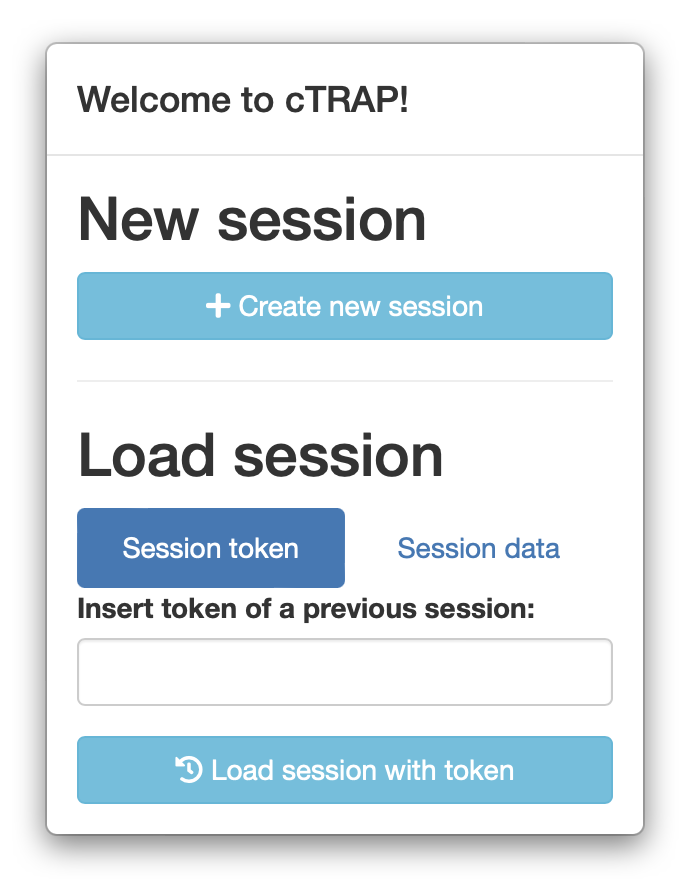
\includegraphics[width=\linewidth]{images/ctrap/welcome}
  \caption[Welcome screen modal]{\textbf{Welcome screen.}}
  \vspace{-\intextsep}
  \label{fig:ctrap-welcome}
\end{wrapfigure}

When visiting cTRAP, a user is greeted with a welcome screen that allows to create a new session or restore a previous one (\autoref{fig:ctrap-welcome}). If the user creates a new session, a random string of numbers and letters is created, henceforth denominated as \emph{token}. The token will be the name of the folder storing user data in the web server and thus cTRAP ensures that token is unique and no other folder is currently using it (\autoref{fig:user-session}).

% TODO: mention other files in common across cTRAP?
If the user loads data to their session, a new folder is named after the session token (\autoref{fig:user-session}). Any changes performed and new datasets appended to the session data are immediately saved to the session folder. The common cTRAP data available across sessions (e.g. the big 21GB CMap perturbations z-scores file) can be made available in a folder accessible to all sessions, thus skipping the step of downloading and preparing the data.\footnote{This is how cTRAP is configured in our web server.}

While using cTRAP, the user can create a new session, load a previous session via a token or a RDS file at any time. When using the token, cTRAP loads the contents of the folder named after the token – if no such folder exists, it will warn the user (\autoref{fig:user-session}). In case the user uploads a RDS file, cTRAP will create a new session and load the contents of the RDS file as the data session (\autoref{fig:user-session}). Using an RDS file ensures the user can open the data in an R session in their local computer given that this RDS file is simply a list of all the datasets available in the session or even use this file in a local version of cTRAP. Moreover, as sessions start to accumulate in our server, they may be removed from the system and thus may become inaccessible\footnote{We have also considered implementing a 14-day expiration date for user sessions. This is not currently in place.}.

\begin{figure}[!ht]
  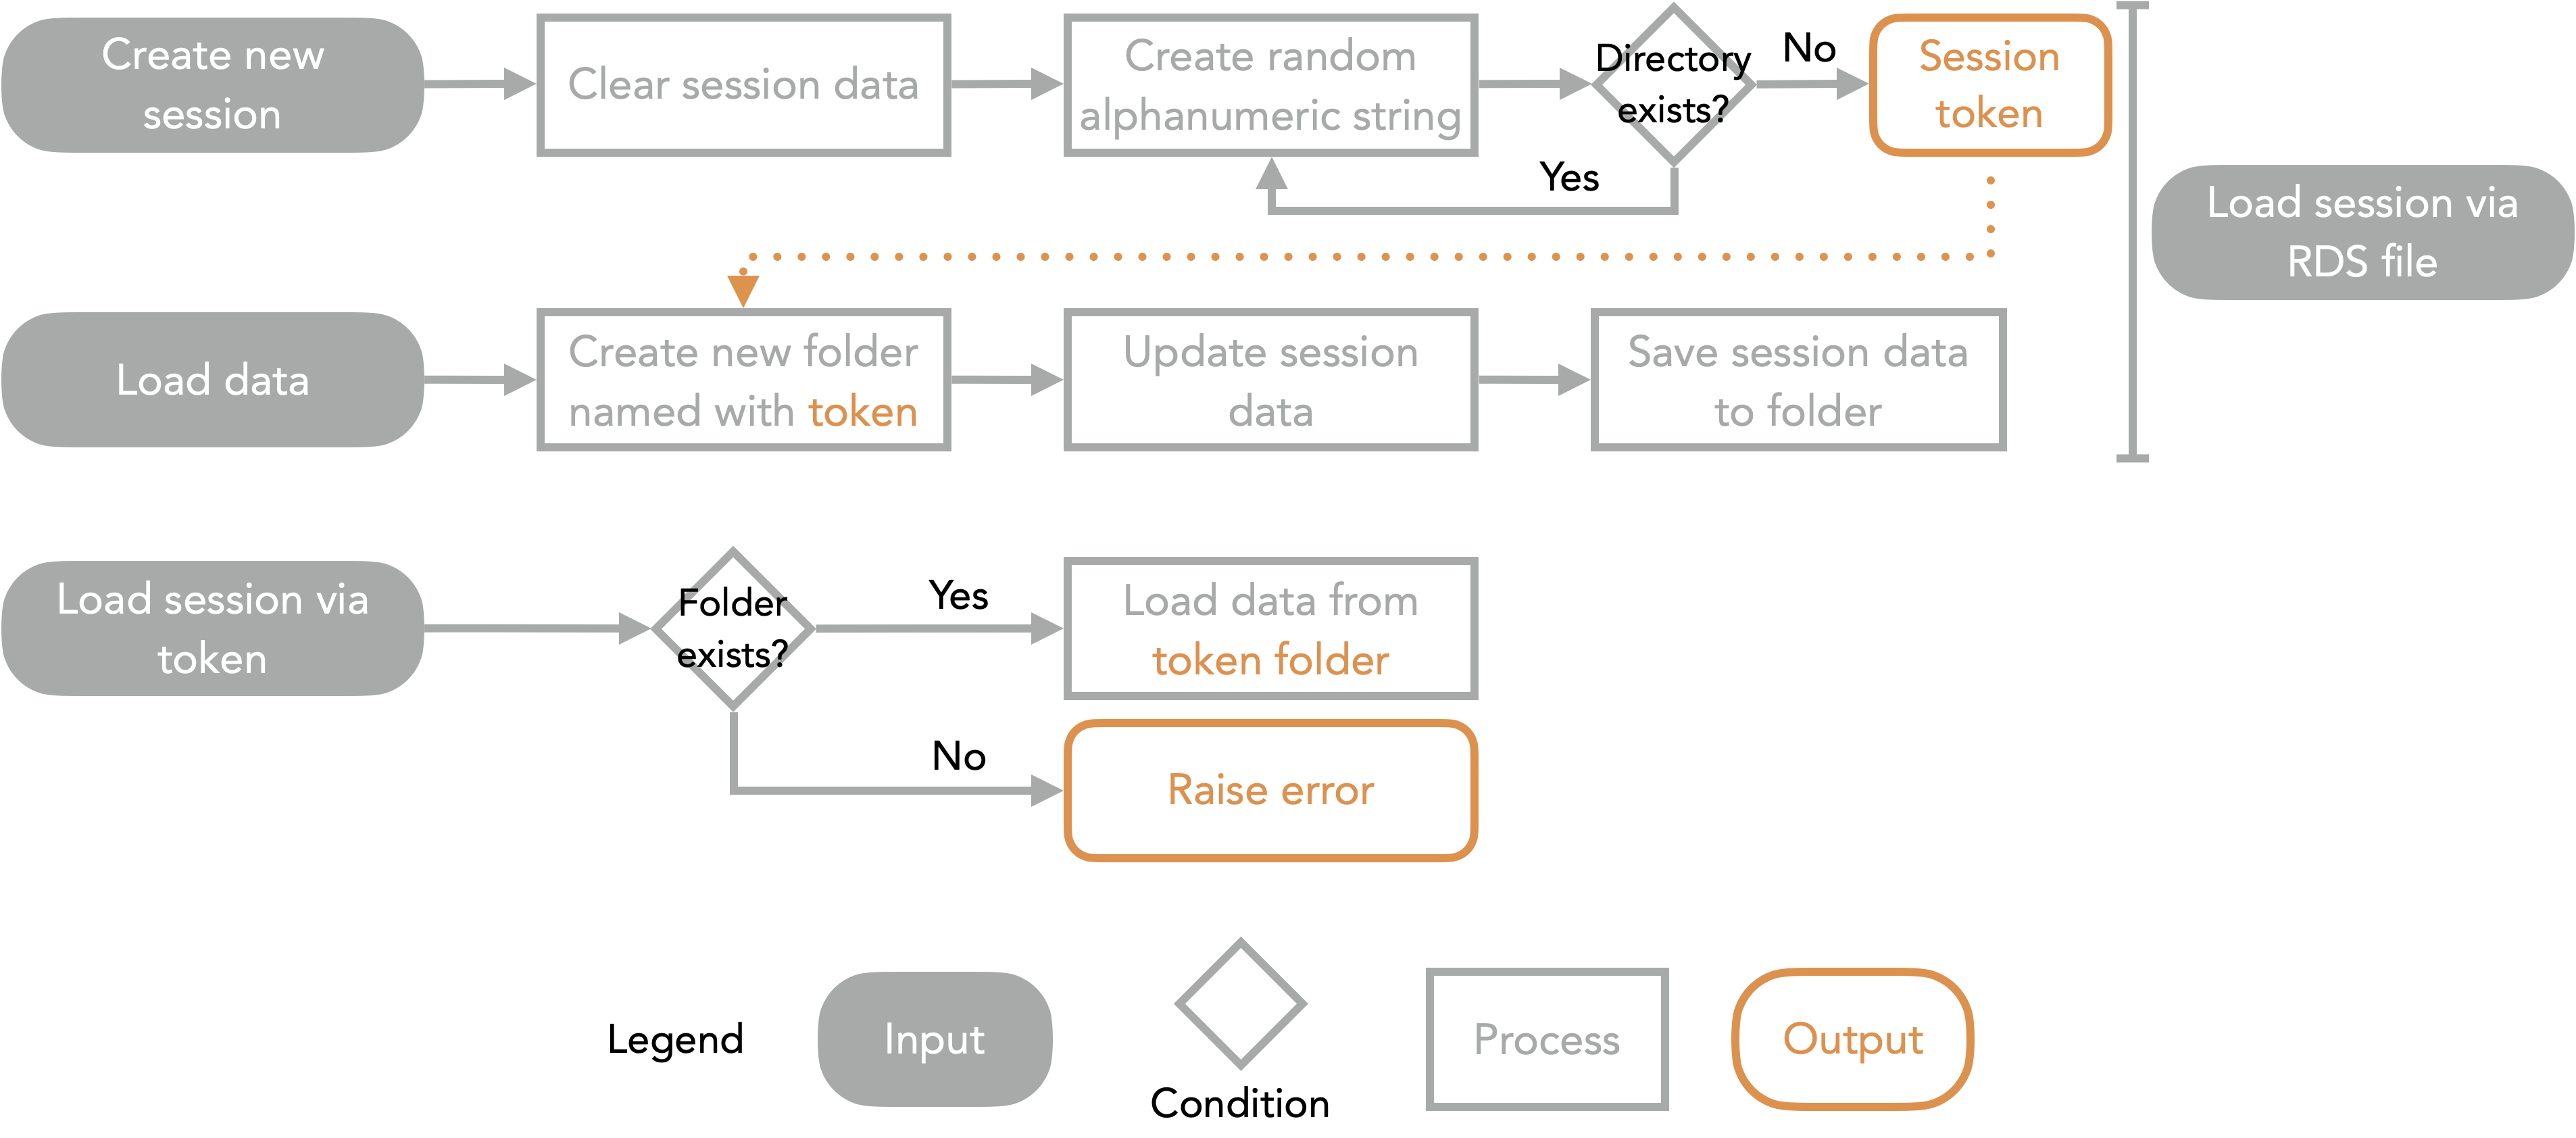
\includegraphics[width=\textwidth]{images/ctrap/user-session}
  \centering
  \caption[User session workflow]{\textbf{User session workflow.} cTRAP allows to create new session or load a previous one via token or RDS file.}
  \label{fig:user-session}
\end{figure}

\subsection{Background tasks}

% TODO: Functions to deal with dummy/mock object

To run tasks in the background, I decided to use Celery, a task queue manager written in Python, and Flower, a Celery monitoring app that also provides a useful RESTful API to work with Celery. Flower makes it easier to send tasks to Celery via HTTP methods, facilitating the communication between cTRAP and Celery. To make use of Flower in R, I created floweRy, an R package to help create the commands used in the Flower API more easily.

If Celery/Flower support is not available, cTRAP can run tasks in the same R process (as usual in an R/Shiny app) so the user has to wait for the long-running tasks to finish before proceeding with interacting with the app. Another limitation is that if cTRAP times out or is shut down, the running processes will stop.

\begin{figure}[!ht]
  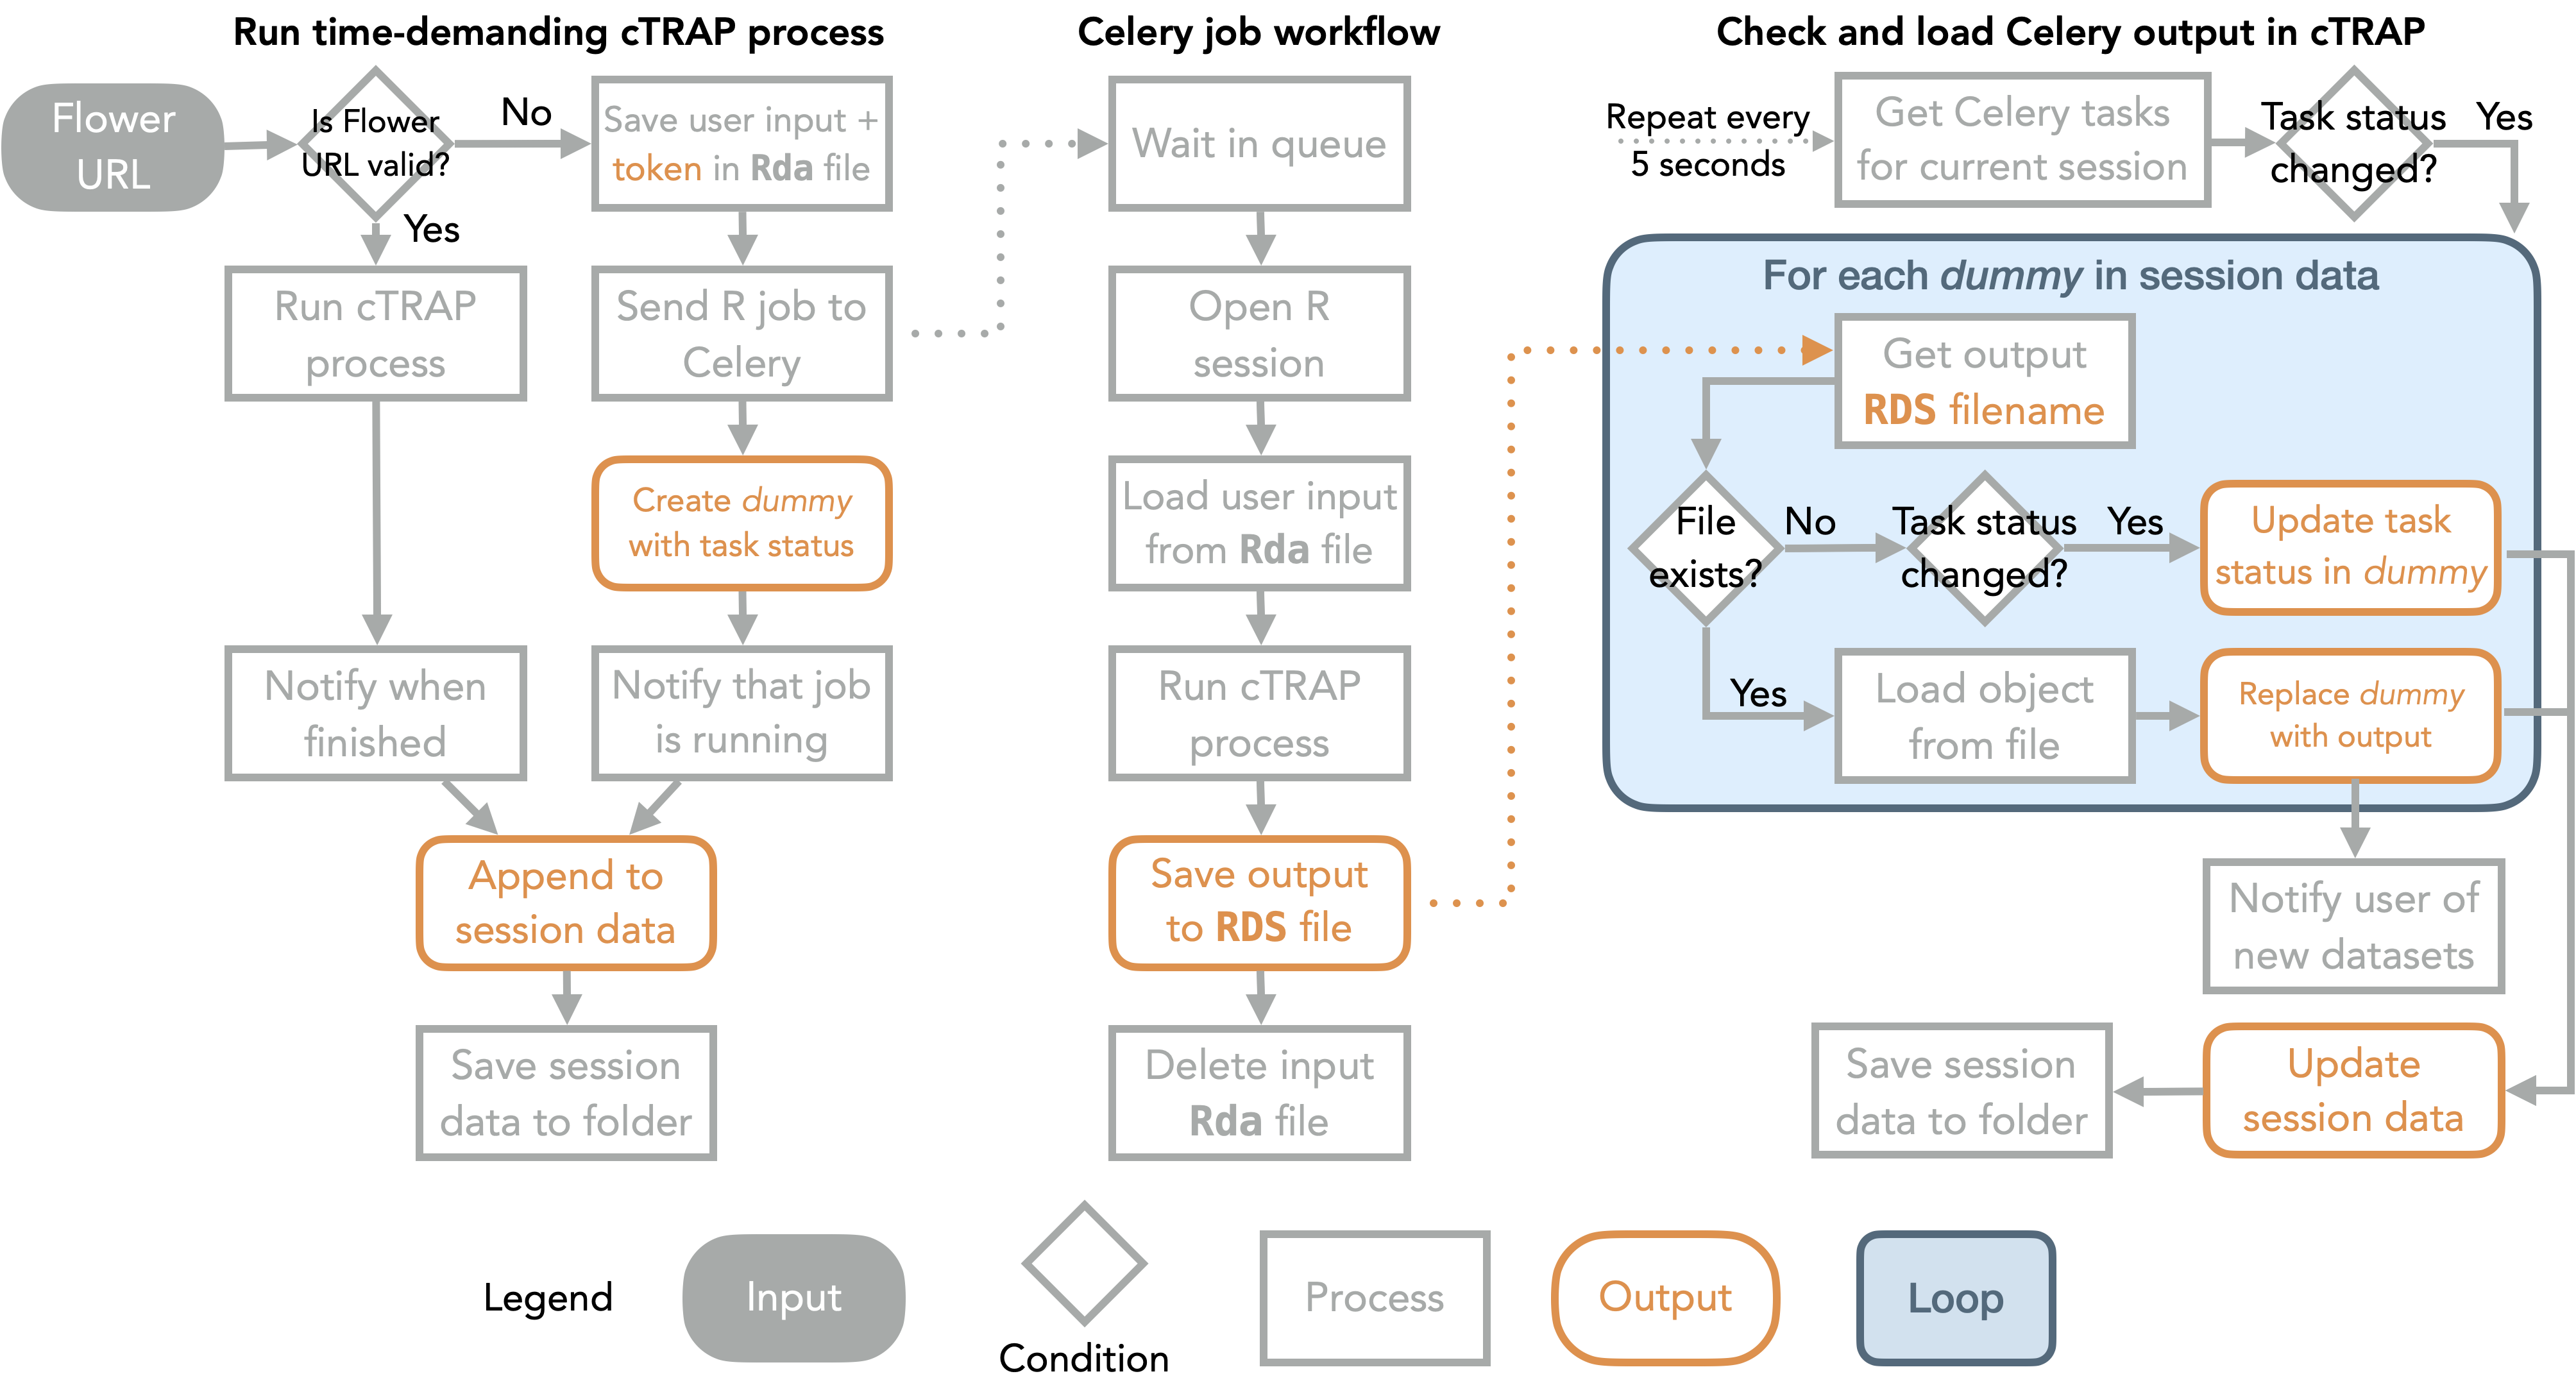
\includegraphics[width=\textwidth]{images/ctrap/celery-job}
  \centering
  \caption[cTRAP process running in Celery]{\textbf{cTRAP process running in Celery.} Time-demanding cTRAP processes can be run in the background using Celery/Flower. While running in Celery, the output of the cTRAP process is saved to the folder associated with the token of the user's session. When that specific session is active, all finished files are automatically loaded as part of the data session and the user is notified.}
\end{figure}

During the whole process, the user interface shows tables with the status of each job from the user. When the process finishes running, the data is automatically loaded and a notification in cTRAP alerts the user that the data is now loaded and ready to visualise.
